\chapter{Application Examples}
\section{F-16 Model}

The flagship use of CSAF is a benchmark F16 fighting falcon model. It serves as an advanced model to develop 
offline and online control assurance schemes. The hope is to provide a benchmark to motivate better 
verification and analysis methods, working beyond models based on Dubins car dynamics, towards the sorts of 
models used in aerospace engineering. Roughly speaking, the dynamics are nonlinear, have about 10-20 
dimensions (continuous state variables), and hybrid in the sense of discontinuous ODEs, but not with jumps in 
the state. \\

A demonstration was created to show how the controllers can be swapped and recompose to alter flight 
trajectories. Figure \ref{fig:f16demoblock} shows an example control system for a \acrlong{gcas} shield.

\begin{figure}[h]
\centering
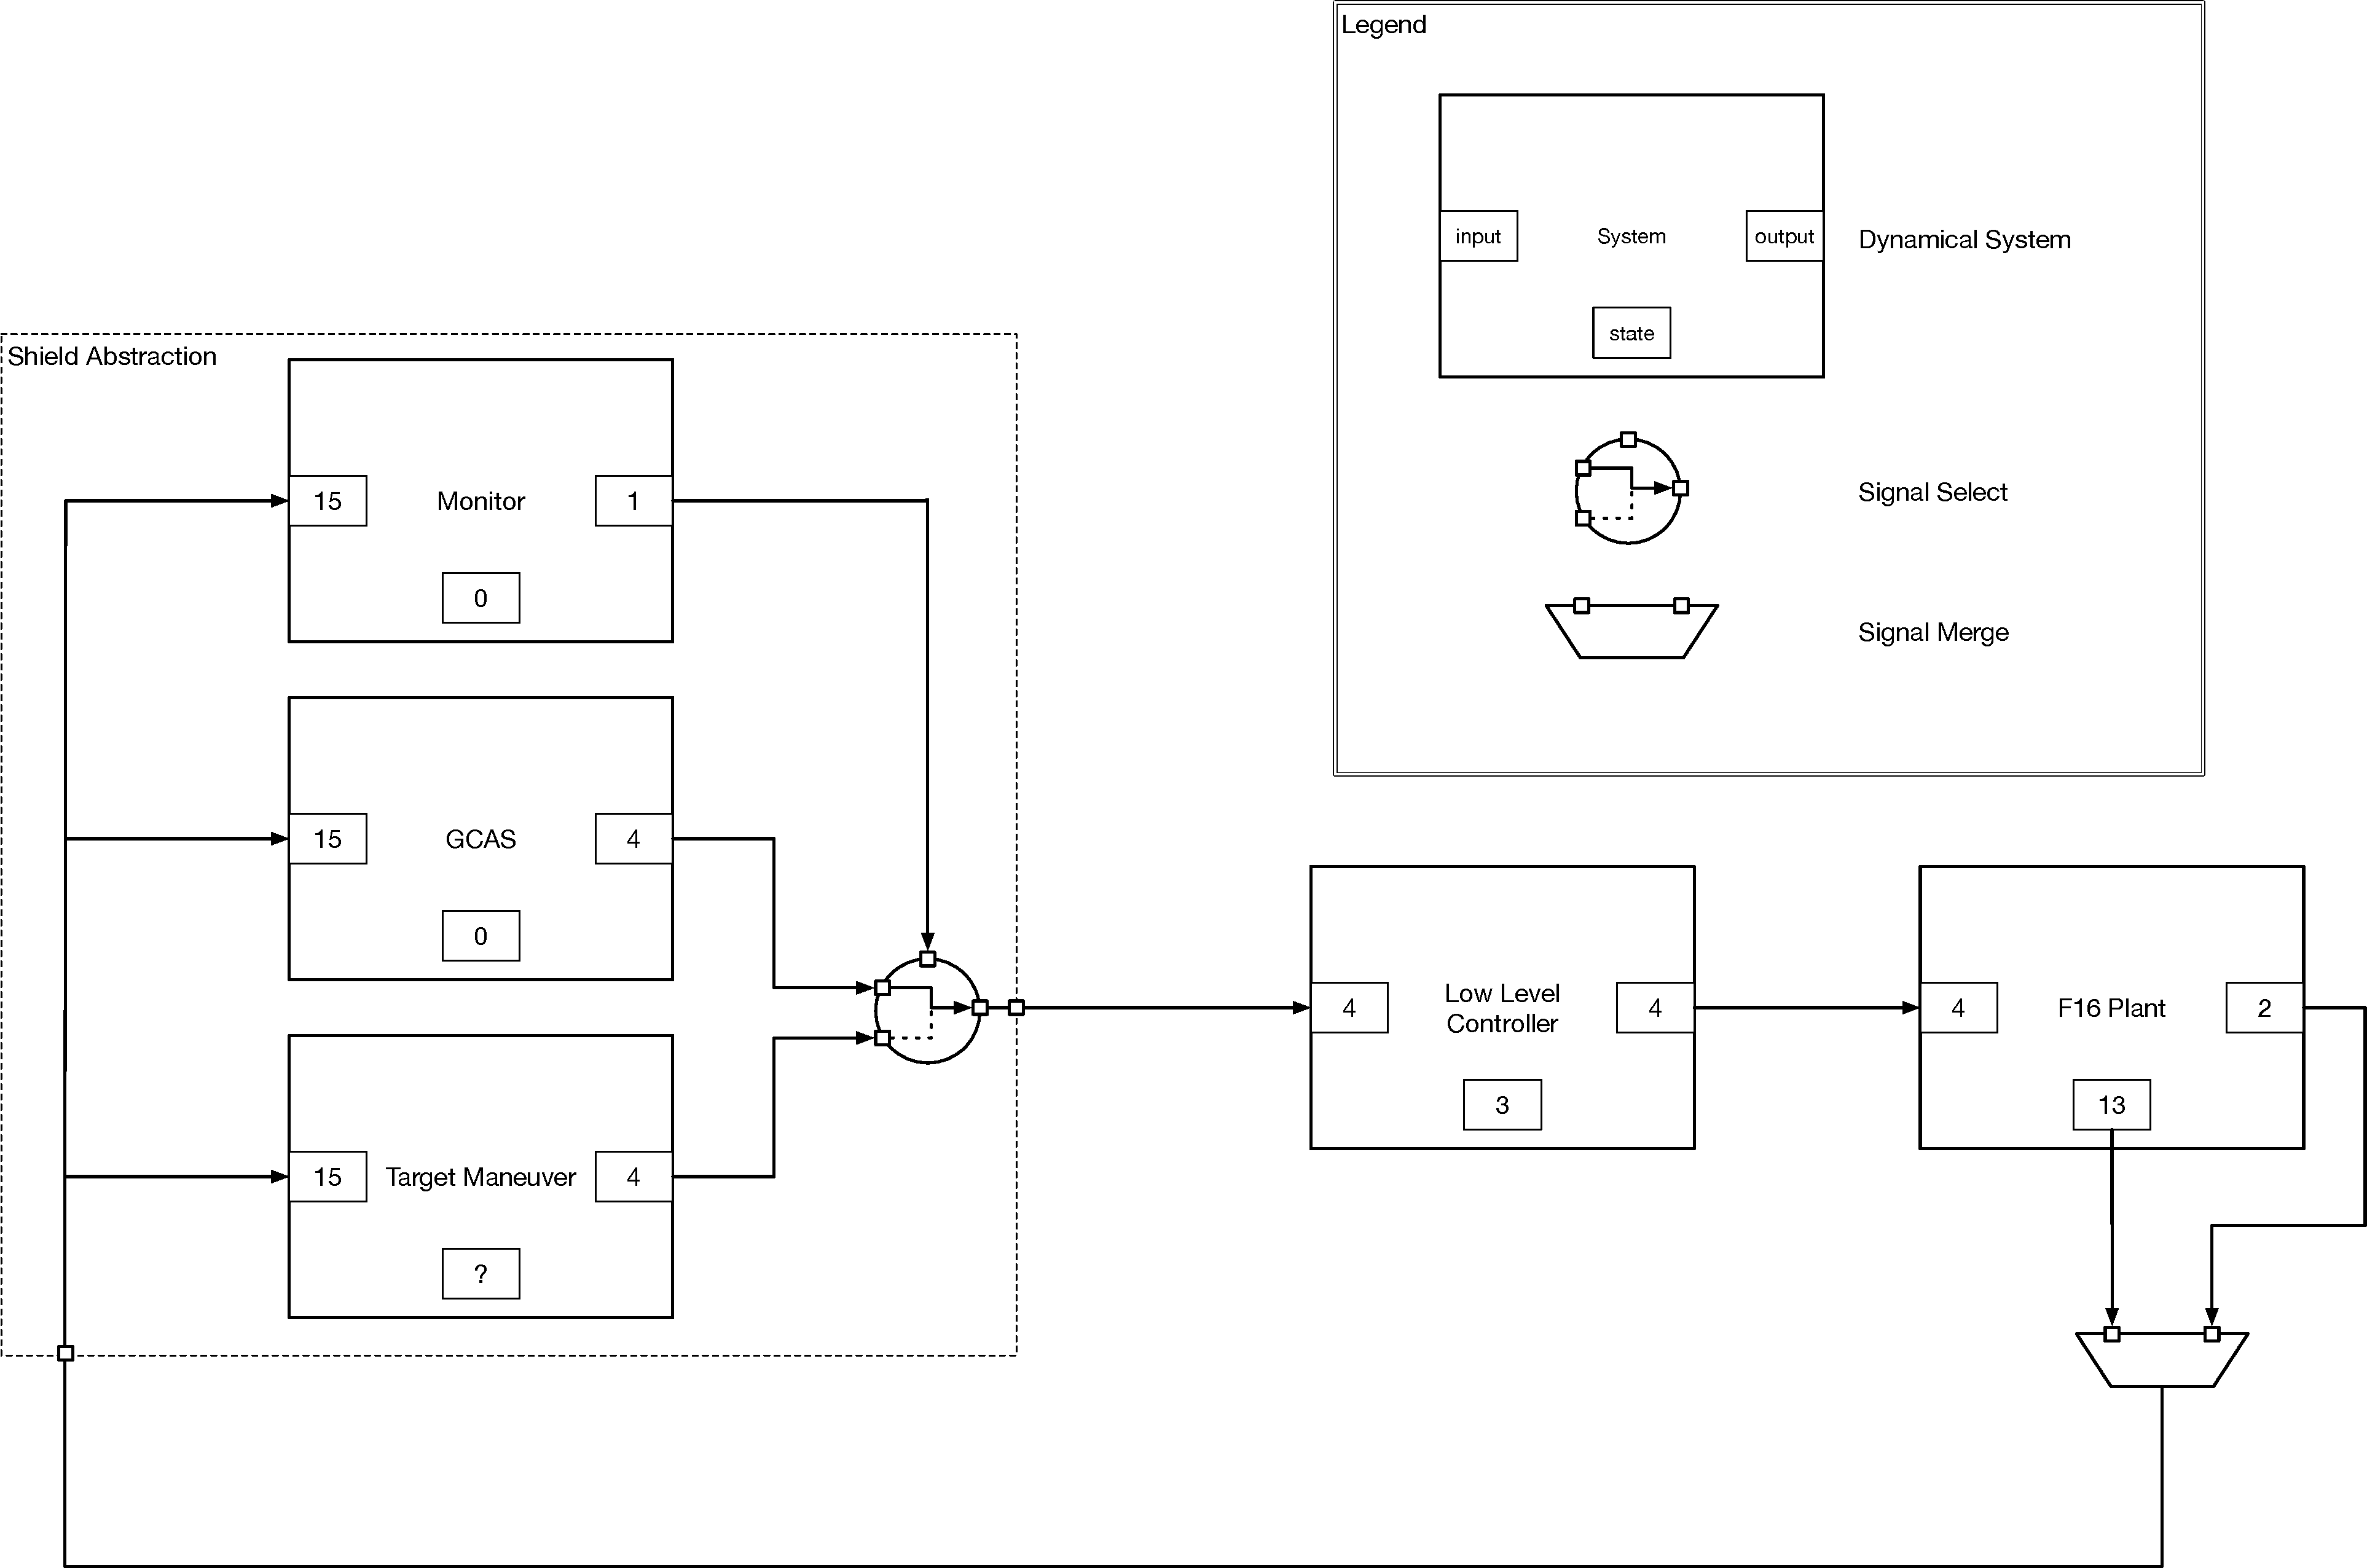
\includegraphics[width=\linewidth]{./img/f16demoblock.pdf}
\caption{Example Shield Configuration for a Controlled F-16 Model Used in Demo}
\label{fig:f16demoblock}
\end{figure}



